\chapter{$\beta$ decay and the weak interaction}
\label{chap:WeakInteraction}

\
Since the electron and the neutrino do not have nuclear interactions, we can assume that their wave function are like the one of free particles
\begin{equation*}
    \psi_e^{-}(\Vec{r}) = \frac{1}{\sqrt{V}}e^{-i\Vec{p}_e\cdot\Vec{r}/\hslash}
\end{equation*}
\begin{equation*}
    \psi_{\hat{\nu}}(\Vec{r}) = \frac{1}{\sqrt{V}}e^{-i\Vec{p}_{\hat{\nu}}\cdot\Vec{r}/\hslash}
\end{equation*}
We have chosen a normalisation such that
\begin{equation*}
    \int_V |\psi_{e^-,\nu}(\Vec{r})|^2\,d\Vec{r} = 1,
\end{equation*}
which means one particle for the volume V. Therefore
\begin{equation*}
    \psi_e(\Vec{r})\psi_{\hat{\nu}}(\Vec{r}) = \frac{e^{-i(\Vec{p}_e+\Vec{p}_{\nu})\cdot \Vec{r}/\hslash}}{V}.
\end{equation*}
The electron and neutrino momentum are typically of the order of 1 MeV/c and we can assume that the wave functions have small variations within the integration volume, $r_0 \sim 1$ fm. Therefore
\begin{equation*}
    \frac{Qr_0}{\hslash} \sim \frac{1\,\mbox{MeV}\,\,\times\,\,1\,\mbox{fm}}{200\,\mbox{MeV}\cdot\mbox{fm}} \sim 10^{-2}.
\end{equation*}
Making an expansion in series
\begin{equation*}
    e^{-i(\Vec{p}_e+\Vec{p}_{\hat{\nu}}\cdot\frac{\Vec{r}}{\hslash}} = 1 - \frac{(\Vec{p}_e + \Vec{p}_{\hat{\nu}})}{\hslash}\Vec{r} - \frac{1}{2}\left(\frac{(\Vec{p}_e+\Vec{p}_\nu)\cdot\Vec{r}}{\hslash}\right)^2 + ..
\end{equation*}
we can approximate the matrix element as 
\begin{equation*}
    \langle f | H_I | i \rangle = \frac{g}{V}\int_{V}\psi_p^*(\Vec{r})\psi_{n}(\Vec{r})\,d\Vec{r},
\end{equation*}
therefore 
\begin{equation*}
    \langle f | H | i \rangle = \frac{g}{V}M_{fi}.
\end{equation*}
The interaction can be generalised to the decay of nuclei 
\begin{equation*}
    _{\tiny{Z}}^{\tiny{A}}N \rightarrow _{\tiny{Z+1}}^{\tiny{A}}Y + e^-+\hat{\nu},
\end{equation*}
with a zero-dimensional operator $O_x$ which can be tuned to reflect experimental data. All the formalism is then equivalent in the two cases
\begin{equation*}
    \langle f | H_I | i \rangle = \frac{g}{V}\int_V \psi_{A,Z+1}^*(\Vec{r})O_x\psi_{A,Z}(\Vec{r}).
\end{equation*}
We can then write in both cases
\begin{equation*}
    \langle f | H_I | i \rangle = \frac{g}{V}M_{fi}.
\end{equation*}

\subsection{Energy density and phase space}
We are considering a three body decay, therefore we need to consider 2 particles in the final state. The number of states for the electron and neutrino can be written as
\begin{equation*}
    dN_e = \frac{V4\pi p_e^2 dp_e}{(2\pi\hslash)^3},
\end{equation*}
and
\begin{equation*}
    dN_{\nu} = \frac{V4\pi p_{\nu}^2 dp_{\nu}}{(2\pi\hslash)^3},
\end{equation*}
therefore the number of possible final states will be
\begin{equation}
    dN = \left[\frac{V4\pi p_e^2 dp_e}{(2\pi\hslash)^3} \right] \left[\frac{V4\pi p_{\nu}^2 dp_{\nu}}{(2\pi\hslash)^3} \right].
    \label{nuclear-physics-eq:1}
\end{equation}
To obtain the energy density of the states, $\rho(E_i)$, let's start from the kinematics of the decay:
\begin{equation*}
    X \rightarrow Y e^- \hat{\nu},
\end{equation*}
where \begin{equation*}
    W = M_X - M_Y = T_Y + E_e + E_\nu,
\end{equation*}
\begin{equation*}
    W = \frac{p^2_Y}{2M_Y} + \sqrt{p_e^2 + m_e^2} + \sqrt{p_\nu^2 + m_\nu^2},
\end{equation*}
and 
\begin{equation*}
    \Vec{p_Y} + \Vec{p}_e + \Vec{p}_{\hat{\nu}} = \Vec{0}.
\end{equation*}
The maximum momentum will be obtained by $Y$ when the electron and the neutrino are emitted in the same direction. Since in the $\beta$ decays the energy $Q$ is typically of the order of 1 MeV, being the mass of the neutrino very small we can take $E_\nu = p_\nu$. Therefore $p$ is very small, and $\frac{p^2}{2M_Y}$ is negligible with respect to $p$. We will have $W \sim E_e + E_\nu$ and therefore
\begin{equation*}
    \begin{split}
        p_\nu^2c^2 & = (W-E_e)^2 - (m_\nu c^2)^2, \\
        p_\nu dp_{\nu} c^2 & = (W-E_e), dW \\
        p_\nu^2 dp_{\nu} c^3 & = (W-E_e)\sqrt{(W-E_e)^2 - (m\nu c^2)^2}. 
    \end{split}
\end{equation*}
We can insert this term in the Equation \ref{nuclear-physics-eq:1}
\begin{equation*}
    dN = \frac{(4\pi)^2V^2}{(2\pi\hslash)^6}\frac{1}{c^3}(W-E_e)\sqrt{(W-E_e)^2 - (m_\nuc^2)^2} \; p_e^2dp_e\; dW,
\end{equation*}
therefore
\begin{equation*}
    \rho(W) = \frac{dN}{dW}
\end{equation*}
can be written as 
\begin{equation*}
    \frac{dN}{dW} = \frac{(4\pi)^2V^2}{(2\pi\hslash)^6}\frac{1}{c^3}(W-E_e)\sqrt{(W-E_e)^2 - (m_\nuc^2)^2} \; p_e^2dp_e.
\end{equation*}
A useful kinematic relation is
\begin{equation*}
    p_e^2 + m^2c^4 = E^2\,\,\rightarrow\,\, 2pdpc^2 = 2EdE,
\end{equation*}
therefore
\begin{equation*}
    pdp = \frac{1}{c^2}EdE.
\end{equation*}
Calling the available energy $W = E_i$, we have
\begin{equation}
    \frac{(4\pi)^2V^2}{(2\pi\hslash)^6c^3}(W-E_e)\sqrt{(W-E_e)^2 - (m_{\nu}c^2)^2} \; p_e E_e dE_e \; \frac{1}{c^2},
\end{equation}
therefore
\begin{equation*}
    \rho(E_i) = \frac{(4\pi)^2V^2}{(2\pi\hslash)^6c^2} E_{\nu} p_{\nu} p_e E_e dE_e \frac{1}{c^2},
\end{equation*}
given that
\begin{equation*}
    p_\nu^2 c^2 = (W-E_e)^2 - (m_\nu c^2)^2,
\end{equation*}
therefore as a function of the kinetic energy of the electron, we have 
\begin{equation*}
    \rho (E_i) = \frac{(4\pi)^2V^2}{(2\pi\hslash)^6c^4} p_e(T_e + m_ec^2)p_\nu E_\nu dT_e,
\end{equation*}
where $T_e = E_e - m_ec^2$.
Applying the Fermi's golden rule we get
\begin{equation*}
    \lambda = \frac{2\pi}{\hslash} |\langle f | H_I | i \rangle |^2 \rho(E_i).
\end{equation*}
Putting all together 
\begin{equation*}
    d\lambda = \frac{2\pi}{\hslash}\frac{g^2}{V^2}|M_{fi}|^2 \frac{(4\pi)^2V^2}{(2\pi\hslash)^6 c^4} p_e(T_e + m_ec^2) \; p_\nu E_\nu dT_e,
\end{equation*}
and calling
\begin{equation*}
    G_F = g(\hslash c)^{-3},
\end{equation*}
we have
\begin{equation*}
    d\lambda = \frac{2\pi}{\hslash} \frac{G_F^2(\hslash c)^6}{V^2}\frac{(4\pi)^2V^2}{(2\pi\hslash)^6c^4} p_e (T_e + m_e c^2) \,
    p_\nu E_\nu dT_e.
\end{equation*}
\begin{figure}[h]
    \centering
    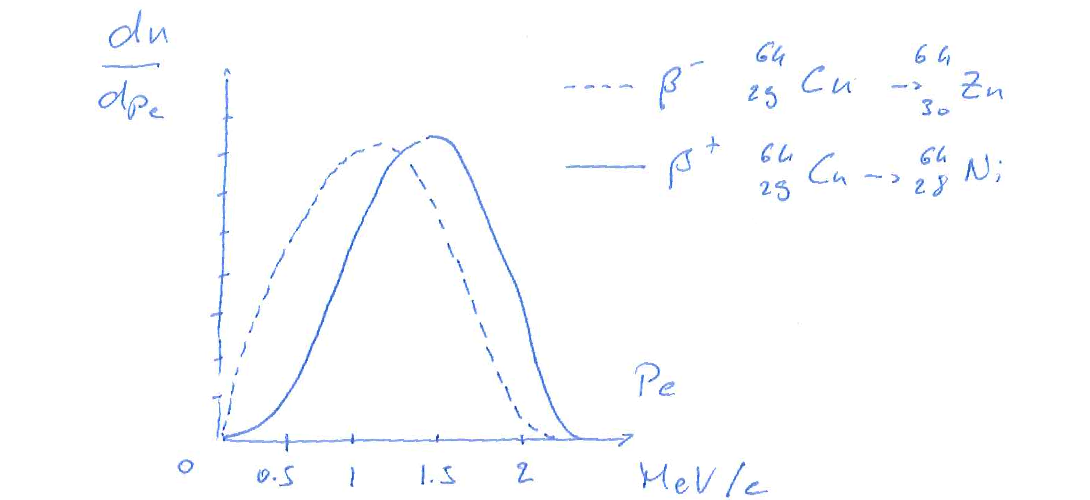
\includegraphics[scale=0.5]{Figures/nuclear-physics-fig20}
    \caption{Momentum distribution of the electron}
    \label{nuclear-physics-fig:20}
\end{figure}
The correction to the matrix element can be denoted as $F(\pm Z, E_e)$, and therefore as a function of the kinetic energy of the electron the shape of the spectrum will be given by
\begin{equation*}
    \frac{1}{\lambda} \frac{d\lambda}{dT_e} \propto p_e (T_e+m_ec^2) p_\nu E_\nu F(\pm Z, T_e).
\end{equation*}
The decay probability can be evaluated through an adimensional integral 
\begin{equation*}
    f(Z,Q) = \frac{1}{(m_ec^2)^5}\int_0^Q p_e c (T_e + m_e c^2) p_\nu E_\nu F(\pm Z, T_e) \, dT_e,
\end{equation*}
therefore in the end we obtain
\begin{equation*}
    \lambda = \frac{G_F^2(m_ec^2)^5}{2\pi^3\hslash}|M_fi|^2 f(Z,Q)
\end{equation*}

\subsection{The neutrino mass}
Analysing in detail the region of the kinematic limit of the distribution of the kinematic energy of the electron in the $\beta$ decay, we observe an interesting dependency at about
\begin{equation*}
    T_e^{max} = Q - m_\nu
\end{equation*}
The energy spectrum is given by
\begin{equation*}
    \frac{d\lambda}{dT_e} = G_F^2 \frac{m_e^5c}{2\pi^3 \hslash} |M_fi|^2 F(\pm Z, T_e) p_e(m_ec^2 + T_e) (Q-T_e) \sqrt{(Q-T_e)^2 - m_\nu^2 c^4}
\end{equation*}
and therefore it is dependant on the mass of the neutrino, as shown in Figure 
\begin{figure}
    \centering
    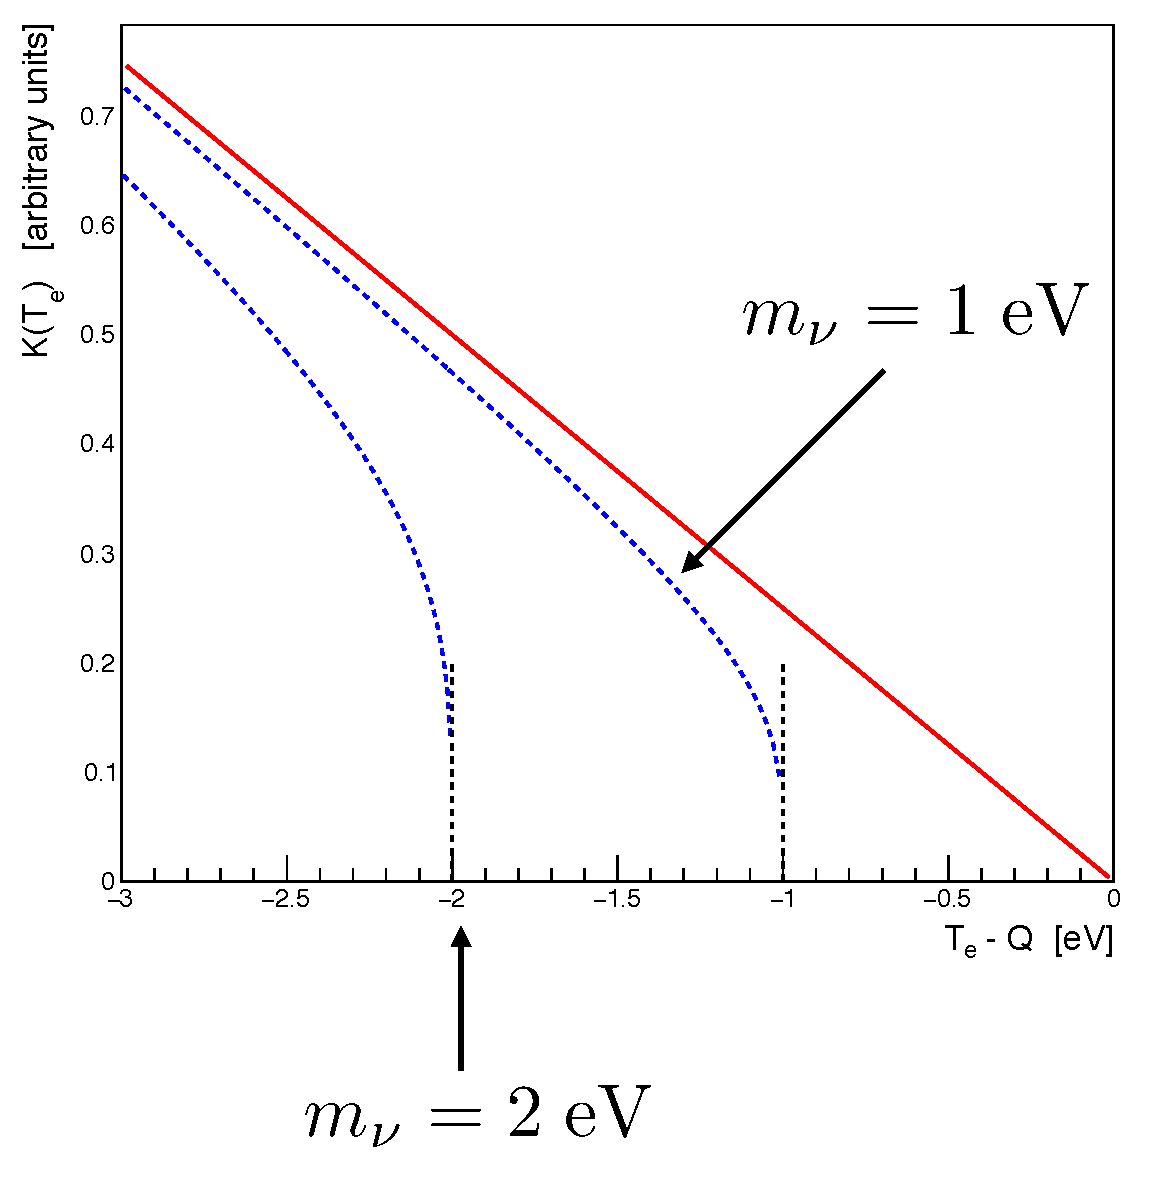
\includegraphics[scale=0.3]{Figures/nuclear-physics-fig21}
    \caption{Endpoint detail for different neutrino masses hypotheses.}
    \label{nuclear-physics-fig:21}
\end{figure}